% !TEX encoding = UTF-8
% !TEX program = pdflatex
% !TEX root = InformationRetrieval.tex
% !TEX spellcheck = it-IT

% 20 Ottobre 2016

% Section Ranking
% Subsection Un modello astratto

% slide 05.20

In ogni caso non c'è un modello di ranking ottimo, perché l'ottimo dipende da cosa vogliamo fornire all'utente.

I modelli visti finora non tenevano conto dell'ordine delle parole e quindi rispondevano allo stesso modo sia a ``\textit{tropical fish}'' che a ``\textit{fish tropical}''.
Per discriminare questi due casi è necessario estendere l'indice in modo che contenga anche la posizione delle parole. Aggiungiamo quindi alle varie posting list dei termini anche la posizione interna del documento in cui compaiono, ottenendo l'indice riportato in figura \ref{fig:index-pos}.

\begin{figure}[htbp]
	\centering
	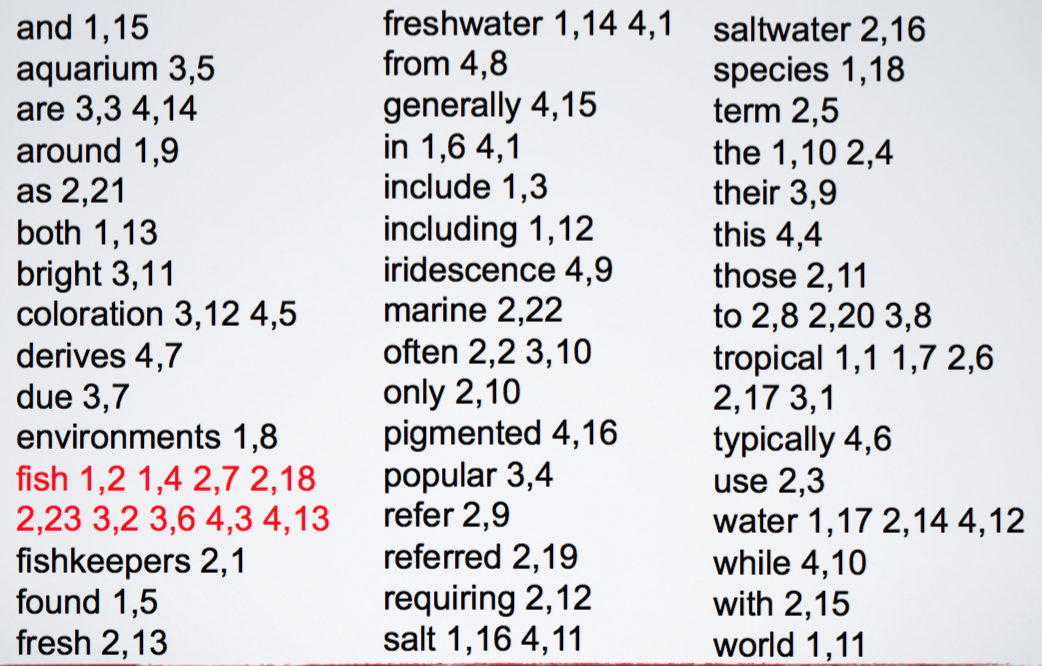
\includegraphics[width=0.6\textwidth]{./images/l7-indice-pos}
	\caption{Indice contenente anche le informazioni relative alla posizione delle parole nei documenti.}\label{fig:index-pos}
\end{figure}

Con questo nuovo indice è possibile è possibile \textit{allineare} le posting list dei due termini e osservare quando il secondo compare subito dopo il primo.
Possono ovviamente capitare dei casi nei quali compare solo uno dei due termini.

Questa tecnica può essere poi estesa per gestire frasi più lunghe oppure utilizzare altri operatori di prossimità: frase esatta, parole ad una certa distanza, ecc.

\subsection{Campi e estensioni}

Tipicamente i documenti, come le email, hanno una certa struttura che fornisce delle informazioni legate al contenuto del documento.

Si può quindi pensare di sfruttare queste informazioni per creare dei sistemi ad-hoc che ad esempio possono implementare degli indici aggiuntivi che contengo le informazioni relative ad un determinato campo.

Un'altra idea è quella di utilizzare un \textbf{extent list}, ovvero una lista che contiene le informazioni relative alle posizioni di inizio e fine dei campi dati d'interesse.
Così facendo è possibile fare il match tra le occorrenze della parola o frase cerca e le informazioni dei campi dati in modo da capire se la parola è contenuta o meno in un determinato campo.

\begin{figure}[htbp]
	\centering
	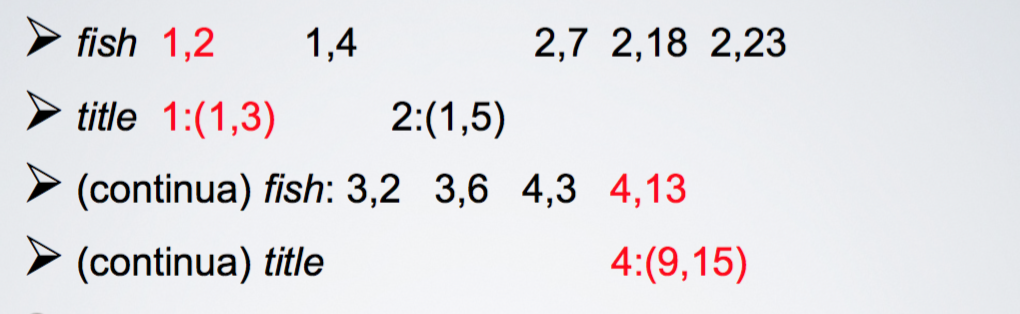
\includegraphics[width=0.6\textwidth]{./images/l7-titoli}
	\caption{Confronto della lista delle posizioni con le posizioni in cui compare un termine. La parola ``\textit{fish}'' compare solamente nel titolo dei documenti \textbf{S1} e \textbf{S4}}
\end{figure}

\subsection{Score nell'indice trasposto}

L'alternativa alla memorizzazione della frequenza è la memorizzazione dello score. 

Tenere lo score può in alcuni casi permettere di risponde più velocemente, perdendo però in flessibilità.

Tipicamente viene quindi preferita la frequenza, tenendo i posting dell'indice ordinati per documento, in modo da facilitare il calcolo dello score.

\chapter{Modelli di reperimento}

Un modello di reperimento dell'informazione è un insieme di costrutti che sono stati ideati e formalizzati allo scopo di rendere possibile la rappresentazione del contenuto dei documenti e delle interrogazioni.

Fa parte del modello anche l'algoritmo di ricerca, ma prima di progettare l'algoritmo è necessario formalizzare il modello di indicizzazione, perché l'algoritmo dipende fortemente dalle informazioni che si hanno riguardo i documenti.

Un modello resta comunque un'astrazione del sistema in quanto è uno strumento che permette di ragionare e rappresentare le sue componenti:

\begin{itemize}
	\item rappresentazione dei documenti;
	\item rappresentazione dell'esigenza informativa espressa nelle interrogazioni;
	\item rappresentazione del funzionamento del sistema.
\end{itemize}

\noindent Non vengono quindi forniti i dettagli implementativi, perché si può sempre pensare di effettuare delle modifiche o di progettare nuove strategie.

\section{Modello IR contro le Basi di Dati}

Nei database il modello ha lo scopo di fornire un'astrazione della rappresentazione del contenuto informativo dei dati e delle operazioni di aggiornamento e accesso ai dati.
Pertanto può succedere che un'utente corrompa i dati presenti oppure che si verifichino situazioni di modifiche concorrenti, ecc.

Nel modello IR non ci sono questi problemi perché le operazioni di aggiornamento vengono effettuate solamente da utenti speciali, mentre le operazioni fatte dagli utenti \textit{normali} sono solo quelle di lettura.

\begin{table}[htbp]
	\centering
	\begin{tabular}{l|l|l|}
		\cline{2-3}
		& Data Retrieval & Information Retrieval            \\ \hline
		\multicolumn{1}{|l|}{Matching}            & Exact match    & Partial/Best match\\ \hline
		\multicolumn{1}{|l|}{Inference}           & Deduction      & Induction                        \\ \hline
		\multicolumn{1}{|l|}{Model}               & Deterministic  & Probabilistic                    \\ \hline
		\multicolumn{1}{|l|}{Classification}      & Monothetic     & Polythetic                       \\ \hline
		\multicolumn{1}{|l|}{Query language}      & Artificial     & Natural                          \\ \hline
		\multicolumn{1}{|l|}{Query specification} & Complete       & Incomplete                       \\ \hline
		\multicolumn{1}{|l|}{Items wanted}        & Matching       & Relevant                         \\ \hline
		\multicolumn{1}{|l|}{Error response}      & Sensitive      & Insensitive                      \\ \hline
	\end{tabular}
\end{table}

A livello di matching, quello effettuato nel IR è sempre parziale, perché viene sempre fornito un sotto-insieme delle informazioni utili all'utente.
Pertanto l'approccio IR è più probabilistico e legato all'induzione, mentre nelle basi di dati il processo di risposta è deterministico.

Un'altra conseguenza di ciò è presente nel query language: per i database è artificiale e molto formale, mentre nei sistemi IR si tratta sempre di un linguaggio artificiale, ma molto più simile a quello naturale, tant'è che in alcuni casi l'utente può fornire le query con il suo linguaggio naturale.

Tipicamente c'è anche una differenza sulle aspettative dell'utente.
Con un database ci si aspetta dei risultati esatti, mentre con i sistemi IR vengono forniti i risultati rilevanti per la query.

\section{Principali modelli}

\begin{itemize}
	\item \textbf{Modello booleano} (1950): il modello più semplice che verifica semplicemente la presenza o meno dell'informazione, senza effettuare l'ordinamento dei risultati. Un esempio di questo modello è dato dai sistemi di ricerca delle biblioteche/archivi.
	\item \textbf{Modello vettoriale} (1960 \textit{Gerald Salton}): modello che tiene conto delle varie feature dei documenti per pesare i risultati, in modo da effettuare l'ordinamento. I primi motori di ricerca si basavano su questo modello.
	\item \textbf{Modello probabilistico} (1970): modello sperimentale ancora poco utilizzato.
	\item \textbf{Modello di analisi della semantica latente} (1980)
	\item \textbf{Modello statistico della lingua} (1990)
	\item \textbf{Modello basato su reti ipermediali} (1980/1990)
\end{itemize}

\section{Modello booleano}

% set di slide 7

In questo modello i descrittori della posting list sono un'insieme di documenti e le interrogazioni sono delle proposizioni logiche in cui gli operandi sono i descrittori, ovvero i termini che compaiono nei documenti.

Le interrogazioni vengono quindi formalizzate utilizzando l'algebra booelana.

\subsection{Documenti di riferimento}

\begin{itemize}
	\item \textbf{D1}: L’enorme quantità di informazioni presenti nelle pagine Web rende necessario l’uso di strumenti automatici per il recupero di informazioni.
	\item \textbf{D2}: I presenti hanno descritto le fasi del recupero dell'enorme relitto ma le informazioni non concordano su tipo e quantità di strumenti in uso.
	\item \textbf{D3}: \`E stato presentato nel Web un documento che informa sulle enormi difficoltà che incontra chi usa uno strumento informativo automatico.
\end{itemize}

\subsection{Indicizzazione nel modello booleano}

I concetti sono rappresentati da descrittori estratti mediante un processo di indicizzazione, quindi un descrittore \textit{t} è l'insieme di tutti e solo i documenti in cui il concetto espresso da \textit{t} è presente.

Effettuando l'indicizzazione vengono quindi perse le informazioni relative alla sinonimia e polisemia.

\begin{itemize}
	\item \textbf{Sinonima}: in linguistica indica la condizione di sostituibilità di un elemento linguistico con un altro nel contesto e nella situazione dati, senza che ne consegue un'alterazione del significato. Fortunatamente la sinonima assoluta è di fatto inesistente nella lingua naturale. Ad esempio se l'utente cerca ``\textit{viso}'' ma tutti i documenti contengo ``\textit{faccia}'' e il modello non gestisce i sinonimi, non vengono trovati risultati.
	\item \textbf{Polisemia}: in linguistica indica la coesistenza in una parola di significati diversi. Ad esempio la parola ``\textit{riso}'' può indicare il riso da risotto oppure l'atto del ridere. Un'altra sfumatura di questo problema sono gli omonimi, \textit{Paolo Rossi} può indicare molte persone ed è quindi necessario disambiguare richiedendo ulteriori informazioni nella query oppure creando altri indici con informazioni utili alla disambiguazione come il codice fiscale o la data di nascita. Per disambiguare in questo caso è possibile utilizzare degli \textbf{authority file}.
\end{itemize}

\subsection{Indice dei descrittori d'esempio}

\begin{figure}[htbp]
	\centering
	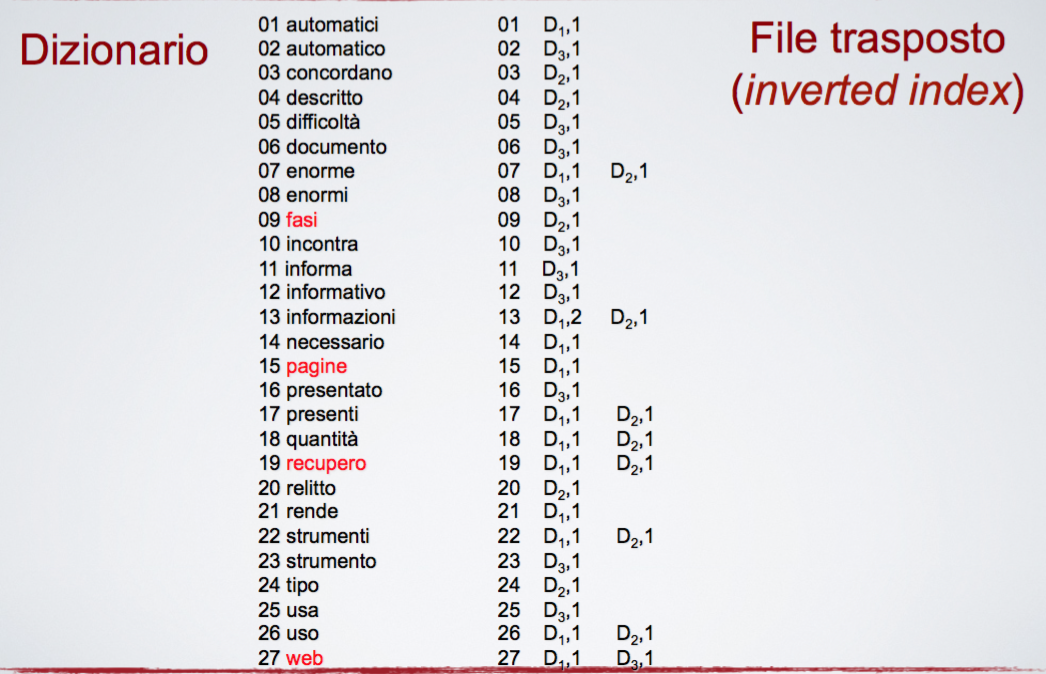
\includegraphics[width=0.6\textwidth]{./images/l7-index-bool}
	\caption{Indice per il modello booleano.}
\end{figure}

C'è da tenere conto che i vari documenti rappresentano un caso ``piccolo'' e quindi nei casi reali l'insieme dei documenti di riferimento è molto più grande.

\begin{figure}[htbp]
	\centering
	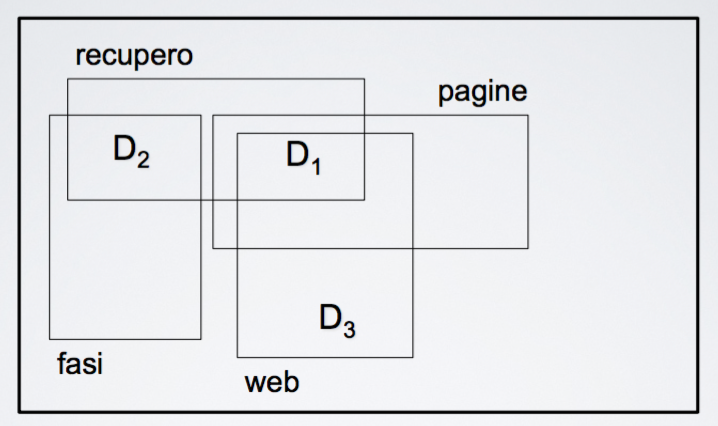
\includegraphics[width=0.6\textwidth]{./images/l7-insieme}
	\caption{Rappresentazione dei documenti sotto forma di insiemi. Sono rappresentati solo alcuni dei termini per questione di spazio.}
\end{figure}

\subsection{Espressione della esigenza informativa}

Un sistema basato sul modello booleano permette all'utente di esprimere le proprie esigenze informative utilizzando più descrittori/termini, i quali vengono utilizzati per costruire l'insieme dei documenti che li contiene.

Se la query è composta da un solo descrittore \textit{x} si parla di una proposizione \textbf{atomica} e vengono forniti in risposta tutti i documenti che contengo il descrittore \textit{x}.

Per combinare i descrittori in modo da definire concetti più complessi vengono utilizzati gli operatori logici: \textit{or}, \textit{and} e \textit{not}.

\begin{itemize}
	\item \textit{or}: richiede che sia presente all'interno del documento almeno uno dei due termini. \`{E} quindi possibile che vengano forniti dei documenti in eccesso.
	\item \textit{and}: richiede che all'interno del documento siano presenti i entrambi i termini. Tipicamente la cardinalità dell'insieme dei documenti fornito è molto minore rispetto a quella dei due insiemi dei termini.
	\item \textit{not}: richiede che il termine non compaia nel documento. Non è però possibile rispondere con tutti i documenti che lo contengono e tipicamente l'utente non vuole tutti i documenti che lo contengo. Questo perché l'utente non ha il concetto di ``\textit{universo dei documenti}''.
\end{itemize}























